%!TEX root = handout.tex

\newpage
\section{Isobaric analysis}
In the last chapters, we identified and quantified the peptides in a label-free experiment. In this section, we would like to introduce a possible workflow for the analyis of isobaric data. We have prepared and copied this workflow to the USB sticks. Please import \directory{Workflows > Identification\_quantification\_with\_inference\_isobaric } into KNIME via the menu entry \menu{File > Import KNIME workflow > Select file} and double-click the imported workflow in order to open it. Before you can execute the workflow, you again have to correct the locations of the files in the \KNIMENODE{Input 
Files} nodes (don't forget the one for the FASTA database inside the ``ID'' meta node). Try and run your workflow by 
executing all nodes at once.

\subsection{Workflow}
Let's have a look at the workflow (see Fig \ref{fig:isobaric_wf})

\begin{figure}[htbp]
  \centering
  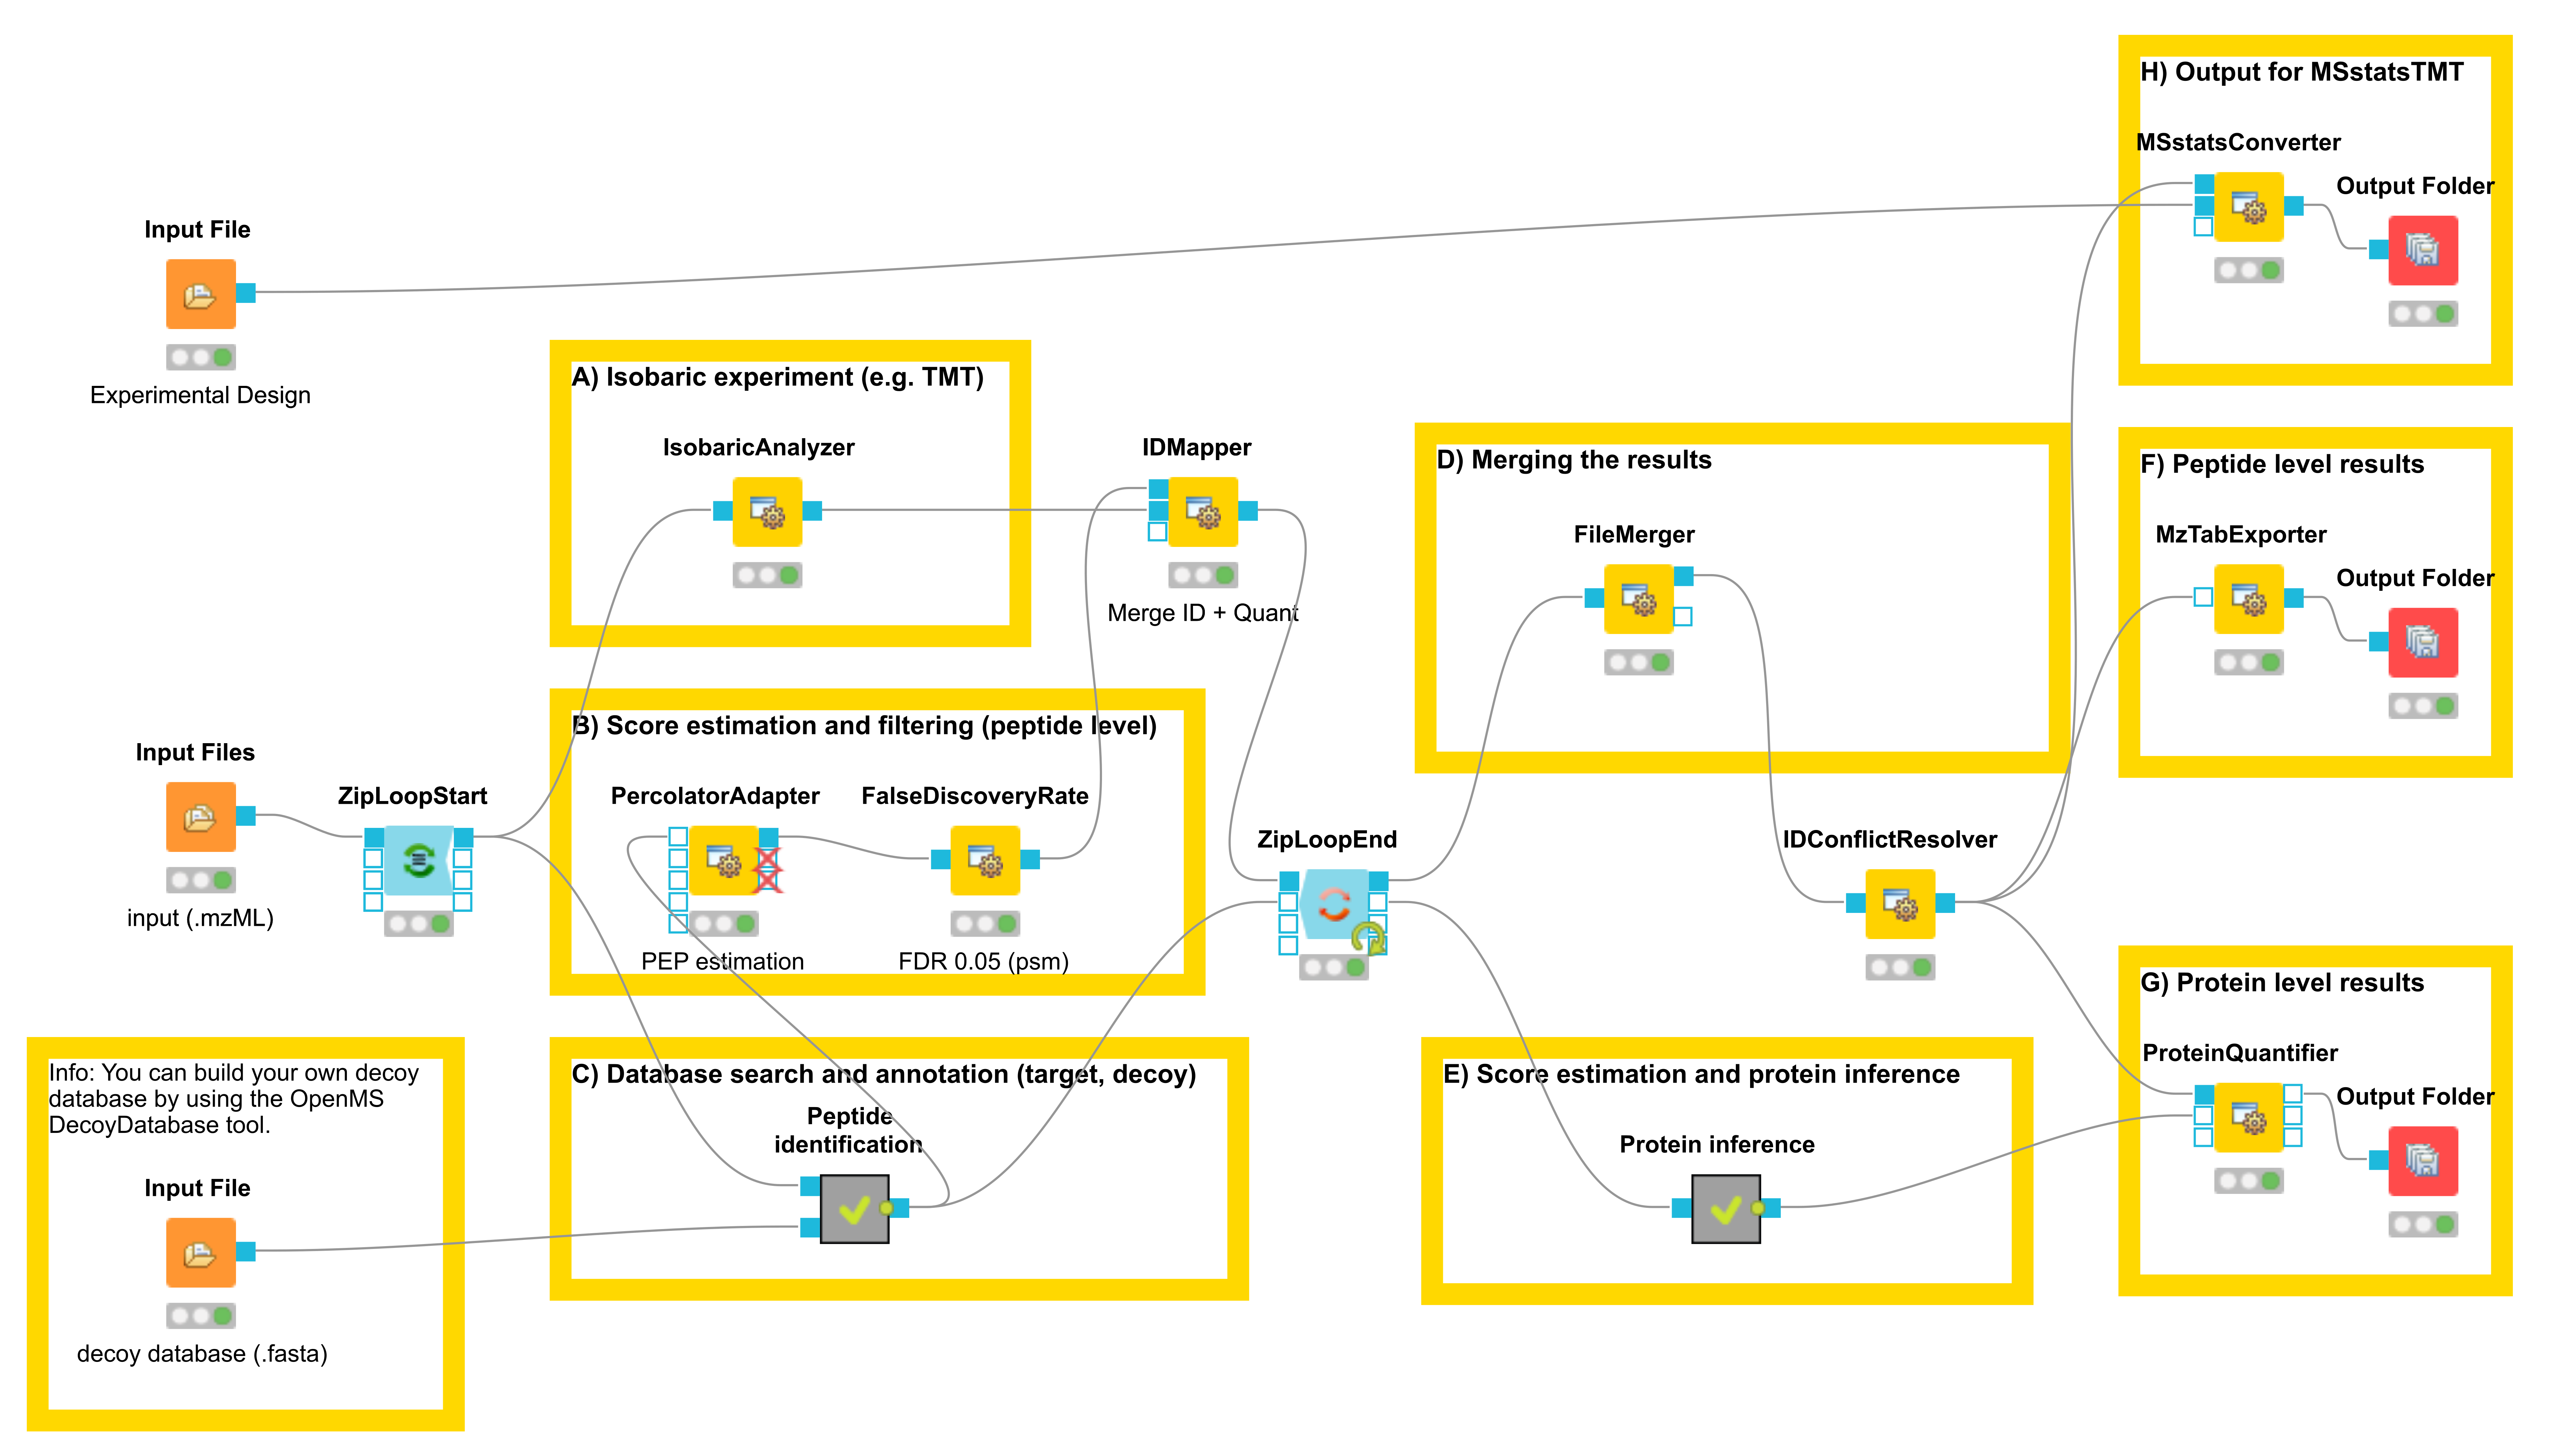
\includegraphics[width=0.95\textwidth]{graphics/isobaric/id_qu_pi_isobaric.png}
  \caption{Workflow for the analysis of isobaric data}
  \label{fig:isobaric_wf}
\end{figure}

There are three input nodes. The first for the experimental design to allow for MSstatsTMT compatible export (.tsv). The second for the .mzML files with the centroided data from the isobaric labeling experiment and the last one for the .fasta database used for identification. The quantification (A) is performed using the \KNIMENODE{IsobaricAnalzyer}. The tool is able to extract and normalize quantiative information from TMT and iTRAQ data. The values can be assessed from centroided MS2 or MS3 spectra and isotopte correction is performed based on the specified correction matrix (as provided by the manufacturer). The identification (C) is performed as known from the previous chapters by using database search and a target-decoy database. 

The workflow is performed on two levels, peptide level (B, D, F, H) and protein level (E, G). On peptide level the posterior error probability (PEP) estimation and FDR filtering is performed on PSM level for each file individually (B). Afterwards the identification (PSM) and quantiative information is combined using the \KNIMENODE{IDMapper}. After the processing of all available files, the intermediate results are aggregated (D) and can be exported via \KNIMENODE{MzTabExporter} (F) or further processed to obtain a MSstatsTMT
compatible version. Here, the R package MSstatsTMT can be used for further processing. \\

This feature is currently only supported for peptide level results. \\

On protein level the identification information over all the files is used to asses the PEP and protein inference is performed using the \KNIMENODE{epifany} (E). The protein and peptide level information is then used by the\KNIMENODE{ProteinQuantifier} to compute the peptide and protein abundances (G).  

\subsection{Experimental Design (TMT)}
We will illustrate the experimental design and the analysis on a subset of the Plubell 2017 dataset (\url{https://github.com/pwilmart/Plubell_2017_PAW; https://www.ebi.ac.uk/pride/archive/projects/PXD005953}), which is a multiplexed TMT labeling experiment to determine age and high fat diets specific proteomie changes in mouse epididymal adipose tissue. It is fairly complex multiplexing 3 TMT experiments with 10 channels each. 











